Gentry's work was a true breakthrough. It not only presented the first, fully homomorphic encryption scheme, but also gave researchers a very powerful tool, the \textit{bootstrapping}. From now on, all we need to construct another FHE scheme, is some suitable (one requirement would be to use a scheme based on ring rather than a group) SHE method, apply appropriate "squashing" to obtain the bootstrapping and we are done. In the following years this is exactly what happened in academia and the industry.

This section will mostly serve as a survey of the main developments towards more efficient fully homomorphic encryption using (ideal) lattices and their security based on computational hardness of the underlying problems. We adopt chronological narrative of the sections, starting with the oldest, the GGH scheme from 1997, progressing through works on (ring-)LWE and eventually arriving at the work of Gentry \cite{gentry_phd} on ideal lattices and further developments on FHE. For a good survey on the lattice based cryptography, see for example \cite{two_faces}, \cite{book} chapter 6 or \cite{lattice-survey}.

\subsection{The GGH public key cryptosystem}
We will start this section with a somewhat simpler cryptosystem that was developed by Goldreich, Goldwasser and Halevi and presented in 1997 \cite{ggh}, called the GGH cryptosystem. This scheme, rather than using ideal lattices (i.e. lattices that are also ideals in the ring of integers), relies on general properties of lattices. Namely, the hardness of the SVP and CVP (see section \ref{hardness}).

\subsubsection*{Idea behind the scheme}
The basic GGH cryptosystem, as mentioned before, is based on the problem of finding the closest vector in the lattice $\mathcal{L}$ to a given point in the ambient space $\R^n$. We are given two bases, call them $\Bg$ and $\Bb$. The $\Bb$ will be our public key and $\Bg$ the secret key. The $\Bb$ consists of long and highly non-orthogonal vectors, as opposed to $\Bg$. Our secret message $\bm{m}$ is represented as a binary vector which we will use to form a linear combination $\bm{s} = \sum m_i \bm{v}_i^{bad} \in \mathcal{L}$ of the vectors in $\Bb$. We now add some small and random error $\bm{e} \in \R^n$ to obtain the ciphertext $\bm{c} = \bm{s} + \bm{e} = \sum m_i \bm{v}_i^{bad} + \bm{e} \in \R^n$ - some point that is not in the lattice, but rather, very close to a point in it.\\
To decrypt, we can use our good basis $\Bg$ to represent $\bm{c}$ and, for example Babai's algorithm\footnote{Simply stated, if the vectors of the basis are sufficiently orthogonal to one another, then this algorithm solves \prob{approxCVP}. However, if the Hadamard ratio is too small, the algorithm fails to find the closest vector - \cite{book}.} to find $\bm{v}$ and represent it in terms of the basis $\Bg$ to recover $\bm{m}$. On the other hand, any eavesdropping adversary that is trying to learn our secret, is left with some bad basis that will be of no help in solving the CVP.

\subsubsection*{GGH construction - concretely}
%\noindent\fbox{%
%    \parbox{\textwidth}{%
The encryption algorithm can be seen in the Table \ref{ggh-enc}.
\begin{table}[ht]
	\centering
	\begin{mdframed}
$\alg{KeyGen}$:
\begin{itemize}
    \item Pick a basis $(\bm{v}_1, \bm{v}_2, \dots, \bm{v}_n) \subset \Z^n$ such that they are reasonably orthogonal to one another - i.e. with small Hadamard ratio. We will associatie the vectors $\bm{v}_1, \bm{v}_2, \dots, \bm{v}_n$ as the $n$-by-$n$ matrix $\bm{V}$ and let $\mathcal{L}$ be the lattice generated by these vectors. This is our good basis $\Bg$ - the \textbf{private key}.
    \item Pick an $n$-by-$n$ matrix $\bm{U}$ with integer coefficients and determinant $\pm 1$ and compute $\bm{W} = \bm{UV}$. The column vectors $\bm{w}_1, \bm{w}_2, \dots, \bm{w}_n$ of $\bm{W}$ are the bad basis $\Bb$ of $\mathcal{L}$ - the \textbf{public key}\footnote{As an alternative, in \cite{hnf}, Micciancio suggested to use the Hermite Normal Form (HNF) of $\Bg$ which essentially provides the worst possible lattice choice from both cryptoanalitical and efficiency point of view.}.
\end{itemize}
$\alg{Encrypt}$:\\
To encrypt a message $\bm{m} = (m_1, m_2, \dots, m_n) \in \Z^n$, choose random small vector $\bm{r} \in \R^n$  and compute $\bm{e} = \bm{mV} + \bm{r}$.\\
$\alg{Decrypt}$:\\
Use Babai's algorithm to compute the vector $\bm{v} \in \Ll$ closest to $\bm{e}$. Finally, compute the $\bm{vW^{-1}}$ to recover $\bm{m}$.
\end{mdframed}
\caption{GGH encryption algorithm}
\label{ggh-enc}
\end{table}


The greatest drawback of GGH is that there were no proofs of security presented along the algorithm, only heuristic assumptions. This motivated researchers to look for possible exploits beased on the choice of parameters. Indeed, this scheme turned out to be insecure for most practical choices of the security parameter only 2 years later, in \cite{break1} and broken completely in \cite{break2}. Nonetheless, the ideas presented there have served as a basis for many schemes that are proven to be secure, like for example LWE, and has led to a plethora of applications.
\subsection{Learning With Errors}
Let us now begin with what went wrong in GGH. Namely, first prove the hardness of a problem, then use it to construct a secure and efficient cryptosystem. In this section we introduce \textit{Learning With Errors} (LWE) problem and the cryptosystem introduced by Oded Regev in \cite{regev} (he won the \href{https://eatcs.org/index.php/component/content/article/1-news/2670-2018-godel-prize}{2018 Gödel Prize} for this work). This very important work in the field of lattice based cryptography is, up to the date, one of the most efficient schemes with an actual proof of security. It has served as a foundation for countless subsequent works in the field. \krzys{provide validation for this statement}

\iffalse
\subsubsection*{Lattices - Part II}

\begin{definition}[Dual]
    For a lattice $\mathcal{L} \subset \R^n$ its $\Z$\textit{-dual} is
    $$ \mathcal{L}^{\vee} = \{ y \in \R^n : y \cdot \mathcal{L} \subset \Z \}.$$
    Here, the $\cdot$ means the usual dot product.
\end{definition}

We simply require that the elements of the dual are precisely those vectors that yield an integer when "multiplied" with an element of our lattice. Note that this is different from our standard definition of a dual. Namely, it is not the orthogonal compliment of our starting space, i.e. not all of the elements of the dual have 0 dot product against the vectors of the lattice.

\begin{example}
    Take $\mathcal{L}= \Z 
        \big(\begin{smallmatrix} 1\\2 \end{smallmatrix}\big) + 
        \Z \big(\begin{smallmatrix} 0\\ 1 \end{smallmatrix}\big)$
        To calculate the dual of $\mathcal{L}$ we need our $y = \big(\begin{smallmatrix}
          a\\b\end{smallmatrix}\big)$ elements to satisfy $a \in \Z$ and $2a + b \in \Z$ which is equivalent to asking $a \in (1/2)\Z$ and so $\mathcal{L}^{\vee} = \big(\begin{smallmatrix}
          1/2\\0
        \end{smallmatrix}\big)\Z + \big(\begin{smallmatrix}
          0\\1
        \end{smallmatrix}\big) \Z$
\end{example}

Note that $\mathcal{L}^{\vee}$ is itself a lattice of the same dimension.
\fi

\subsubsection*{LWE problem}
There are multiple equivalent definitions of this problem. We adopt the notation and approach introduced in the original paper by Regev. In this section, we will mainly focus on the parts that are the most relevant for our study of ring-LWE such as\krzys{finish the lemmas most influenced by switch to ring}. 

The problem is parametrized by positive integers $n$, $m$\footnote{As will be seen later, $m$ plays virtually no role in the problem definition and is usually omitted.} and prime $q$, as well as an error distibution $\chi$ over $\Z_q$. It is now defined as follows. We are given $m$ equations of the form $(\bm{a}_i, b_i = \langle \bm{a}_i, \bm{s} \rangle + e_i)$ and are asked to find the vector $\bm{s} \in \Z_q^n$. Here, $\bm{a}_i$ are chosen uniformly and independently from $\Z_q^n$, $b_i \in \Z_q$ and $\langle \cdot, \cdot \rangle$ denotes the usual dot product. The errors $e_i$ are obtained by sampling independently from the probability distribution $\chi : \Z_q \rightarrow \R^{+}$ on $\Z_q$. We will denote the problem of recovering $\bm{s}$ from such equations, by $\text{LWE}_{q, \chi}$ (learning with errors).

\begin{example}\label{lwe_ex}
	Given as input this set of equations, LWE asks us to recover the vector $\bm{s} = (s_1, s_2, s_3, s_4) \in \Z_{17}^4$. In this case $n = 4$, $q=17$ and the error distribution is giving us $e_i < 1$ for each $i \in [m]$. 
\begin{align*}
	0s_1 + 11s_2 +8s_3 + 2s_4 & \approx_{e_1} 3 \, (\mod 17)\\
	9s_1 +  3s_2 + 7s_3 + 0s_4 & \approx_{e_2} 16 \\
	1s_1 +  15s_2 + 9s_3 + 5s_4 & \approx_{e_3} 16 \\
	0s_1 +  0s_2 + 13s_3 + 5s_4 & \approx_{e_4} 1\\
\end{align*}
In this case, $\bm{s} = (7, 13, 12, 16)$. Note that if not for the error, the secret would be very easy to find. Given about $n$ equations, we could recover $\bm{s}$ in an efficient way using Gaussian elimination. Inducing the error is what seems to render the problem untraceable for modern day algorithms.
\end{example}
The central part of \cite{regev} revolves around proving the hardness of LWE. Specifically, that for appropriately chosen $q$ and $\chi$, a \textit{quantum}\footnote{In fact, quantum reduction is used only in the small part of the whole proof.} reduction algorithm exists that approximates worst-case lattice problems. The following is the main result presented in the paper. 

\begin{theorem}[\cite{regev}, Theorem 1.1]\label{main}
	Let $n$, $q$ be positive integers and $\alpha \in (0, 1)$ be such that $\alpha q > 2 \sqrt{n}$. If there exists an efficient algorithm that solves $\text{LWE}_{q, \Psi_{\alpha}}$, then there exists an efficient quantum algorithm that approximates the decision version of the shortest vector problem (\prob{GapSVP}$_{\gamma}$) and the shortest independent vectors problem (\prob{SIVP}$_{\gamma}$) to within $\gamma = \tilde{O}(n/\alpha)$ in the worst case on any lattice of dimension $n$.	
\end{theorem}

Let us unwrap this statement. As said before, we need an appropriate choice of paramenters to obtain our results and $\alpha > 2\sqrt{n}/q$ is one of those choices (and requirements). It specifies the shape of the $\Psi_{\alpha}$ distribution. This one is almost identical to the discrete Gaussian distribution over $\Z_q$ that is centered around 0 with standard deviation $\alpha q$\footnote{A comment from \cite{lattice-survey}: Originally, Regev considered the continuous Gaussian and rounded the result to the nearest integer. This does not exactly yield the discrete distribution but thanks to \cite{discr} we know how the problem can be fixed.}. The theorem can be rephrased as follows. Imagine that we have an efficient algorithm that solves the $\text{LWE}_{q, \bar{\Psi}_{\alpha}}$. Then, there exists a quantum solution to worst-case lattice problems, namely \prob{GapSVP} and \prob{SIVP}. Since we strongly believe that \prob{GapSVP} and \prob{SIVP} are difficult to solve (\cite{svp-hard}, \cite{reductions}, \cite{cvp-hard}) we are left with a difficult, yet efficient way to share secrets. Oded Regev proceeds to prove this using various lemmas and results from few areas of mathematics like probability, lattice theory and quantum computing. We will now present selected proofs and outline of whole the approach.

\subsubsection{Background II}
\paragraph{Gaussians}
\begin{definition}[Statistical distance]
\end{definition}
\paragraph{Problems}
\begin{definition}[Search-LWE]
\end{definition}
\begin{definition}[Decision-LWE]
\end{definition}
\begin{definition}[LWE distribution]\label{lwe-distr}
    Let $q \geq 2$ be some integer, and let $\chi : \Z_q \rightarrow \R^+$ be some probability distribution on $\Z_q$. Let $n$ be an integer and let $\bm{s} \in \Z_n^q$ be a vector. We define $A_{\bm{s},\chi}$ as the distribution on $\Z_n^q \cross \Z_q$ obtained by choosing a vector $\bm{a} \in \Z_q^n$ uniformly at random, choosing $e \in \Z_q$ according to $\chi$, and outputting $(\bm{a}, \langle \bm{a}, \bm{s} \rangle + e)$, where additions are performed in $\Z_q$, i.e., modulo $q$. In parallel, we define $U$ as the uniform distribution on $\Z_q^n \cross \Z_q$.
\end{definition}
\begin{definition}\label{dgs}
\end{definition}
\paragraph{Smoothing parameter}

\subsubsection{Hardness of search LWE}
In this section we will focus on proving the main statement of \cite{regev} following the steps presented in the paper. We will put an emphasis on the parts that require the most adjustment when trying to prove the same results for ring-LWE in the next section.

Recall that we want to prove, that being able to solve $\text{LWE}_{q, \chi}$ implies that we are able to solve standard worst-case lattice problems like \prob{SIVP}. To achieve this, we need to proceed in steps, in other words, we perform reductions from one problem to another. From this point on, a probabilistic algorithm which solves a given $\text{LWE}_{q, \chi}$ instance, will be called an LWE-\textit{oracle} (or, when there is no confusion, simply an oracle).

The high-level version of the proof is as follows. Let us assume that we have such an oracle that solves $\text{LWE}_{q, \chi}$ on a lattice $\Ll$ just like in the assumption. The procedure is based on the so called \textit{iterative step} (IS). It is repeatedly used to reduce our LWE problem to the problem of sampling from the  discrete Gaussian distribution on $\Ll$. As it turns out, it is indeed sufficient to solve the \prob{DGS} problem (Definition \ref{dgs}). Intuitively, if we have enough samples from the Gaussian distribution of some small radius $r$ around our lattice, we can use it to obtain short lattice vectors. Indeed, if we call the \prob{DGS} oracle enough times we can prove, that with very high probability, there are $n$ linearly independent vectors among the samples returned by oracle - thus, a solution to \prob{SIVP}.

On each of the iterations, the IS is using the oracle to produce discrete Gaussian samples of smaller and smaller radius around our desired \textit{closest vector}. Once we have a sample with radius small enough, we can use that to solve \prob{DGS} and use one more step which is the reduction from \prob{DGS} to the \prob{GapSVP} and \prob{SIVP} as required in Theorem \ref{main}.

\begin{center}
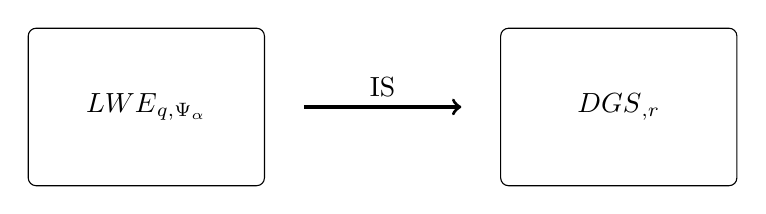
\begin{tikzpicture}
% Define the left box
\draw[rounded corners=1mm] (0,0) rectangle (3,2);
\node at (1.5,1) {$\text{LWE}_{q, \Psi_{\alpha}}$};

% Define the right box
\draw[rounded corners=1mm] (6,0) rectangle (9,2);
\node at (7.5,1) {$\text{DGS}_{\Ll, r}$};

% Define the arrow between the boxes
\draw[->, very thick] (3.5,1) -- node[above] {IS} (5.5,1);
\end{tikzpicture}
\end{center}

The algorithm can be divided into two basic steps, the \textit{classical} step and the \textit{quantum} step. First, given some polynomial number $n^c$ (where $c$ is some positive integer) of samples from a discrete Gaussian on $\Ll$ with some (large enough) parameter $r$, we us the first step to obtain a solution to a \prob{CVP} on the dual lattice $\Lld$ to within some (smaller than the initial $r$) distance. We then use this solution along with the second step - the quantum algorithm - to obtain $n^c$ samples from a dicrete Gaussian with parameter $r' < r$. Iterating these steps polynomial amount of times, we finally get $n^c$ samples from D$_{\Ll, r''}$ where $r'' \ll r$. We simply pick one of those samples to solve the DGS$_{\Ll, r}$ and we are done.
\krzys{input a schematic as nice as the one in regev}\\
The full picture now stands as follows. We begin with a assumed solution to LWE and we end up with a solution to some (conjured) hard lattice problems like SIVP to within some tolerance $\gamma$.
\begin{center}
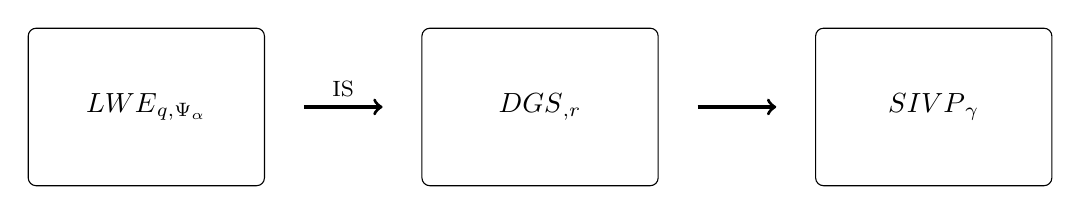
\begin{tikzpicture}
\draw[rounded corners=1mm] (0,0) rectangle (3,2);
\node at (1.5,1) {$\text{LWE}_{q, \Psi_{\alpha}}$};

\draw[->, very thick] (3.5,1) -- node[above] {\footnotesize IS} (4.5,1);

\draw[rounded corners=1mm] (5,0) rectangle (8,2);
\node at (6.5,1) {$\text{DGS}_{\Ll, r}$};

\draw[->, very thick] (8.5,1) --  (9.5,1);

\draw[rounded corners=1mm] (10,0) rectangle (13,2);
\node at (11.5, 1) {$\text{SIVP}_{\gamma}$};

\end{tikzpicture}
\end{center}
We will now focus on the first step of the reduction from LWE to \prob{DGS} as it is what is altered the most in the ring-LWE hardness proof. This, however, will follow in the next section.

The following statement (Theorem 3.1 in \cite{regev}) is the core of the hardness results of (search) LWE. Given an oracle form LWE, there exists an algorithm that gives us samples from discrete Gaussian distribution which in turn can yield us a solution to the \prob{CVP}. For example, later we will show the equivalence between search-LWE and decision-LWE (Theorem \ref{s-to-d}). This is an important result as it is usually much easier to construct cryptographic schemes based on some \textit{decision} version of a problem rather than the \textit{search}.

\begin{theorem}\label{heart}
	Let $\epsilon = \epsilon(n)$ be some negligible function of $n$. Also, let $q = q(n)$ be some integer and $\alpha = \alpha(n) \in (0, 1)$ be such that $\alpha q > 2\sqrt{n}$. Assume that we have access to an oracle W that solves $\text{LWE}_{q,\Psi_{\alpha}}$ given a polynomial number of samples. Then there exists an efficient quantum algorithm for $\text{DGS}_{\sqrt{2}n \cdot \eta_{\epsilon}(L)/\alpha}$.
\end{theorem}
\begin{proof}
	The proof follows in a straight-forward manner by the Lemma \ref{is}. We sample a polynomial amount of elements from the D$_{\Ll, r}$ for $r$ large enough\footnote{By Claim 2.13 and Lemma 3.2 of \cite{regev}, we can efficiently draw samples that are exponentially close to D$_{\Ll, r}$ if $r > 2^{2n} \lambda_n(\Ll)$.}. We then apply the IS to obtain D$_{\Ll, r'}$ for $r' \leq r/2$. Applying this procedure enough times (turns out only about $3n$ iterations are needed). At the end of the loop, we are left with the same amount of samples but each within sufficient distance $d \leq \sqrt{2}n \cdot \eta_{\epsilon}(\Ll)/\alpha$ and we complete the algorithm by simply outputting the first one.
\end{proof}

\paragraph{The iterative step}
The proof of Theorem \ref{heart} relies mainly on the following algorithm. This is slightly altered Lemma 3.3 in \cite{regev}. 
\begin{lemma}[Iterative Step]\label{is}
	Let $\epsilon = \epsilon(n)$ be a negligible function, $\alpha > 0$ real, and $q \geq 2$ be an integer. Assume that we have access to an oracle that solves $LWE_{q,\Psi_{\leq \alpha}}$ given a polynomial number of samples. Then, there exists an efficient quantum algorithm that, given any $n$-dimensional lattice $\Ll$, a number $r > \sqrt{2}q \eta_{\epsilon}(\Ll)$, and a polynomial list of samples from the discrete Gaussian distribution $\text{D}_{\Ll,r}$, produces a sample from $\text{D}_{\Ll,r\sqrt{n}/(\alpha q)}$.
\end{lemma}
\begin{proof}
	As mentioned before, the algorithm consists of two parts. The first part is presented in \ref{classical}, where, given an oracle W and samples from $\text{D}_{L,r}$, solves \prob{CVP}$_{L^{\vee}, \alpha q / (\sqrt{2} r)}$. The second part - the quantum algorithm \ref{quantum} - when given an oracle that solves \prob{CVP}$_{L^{\vee}, \alpha q / (\sqrt{2} r)}$, yields us a sample from $\text{D}_{L, r\sqrt{n}/\alpha q)}$.
\end{proof}

Pictographically, here are two iterations of the algorithm:
\krzys{include pictoraphic like in Regev page 8}

We now present heavily simplified version of the algorithm that, when given a polynomial amount of samples from the discrete Gaussian, gives us a solution to the \prob{CVP} to within error of $\alpha q /(\sqrt{2} r)$ to the dual lattice $\Lld$.
\begin{lemma}[Step 1 - classical]\label{classical}
	Let $\epsilon = \epsilon(n)$ be a negligible function, $\alpha > 0$ real, and $q \geq 2$ be an integer. Assume that we have access to an oracle that solvesLWE$_{q, \Psi_{\leq \alpha}}$ given a polynomial number of samples. Then, there exists an efficient algorithm that given an $n$-dimensional lattice $\Ll$, a number $r > \sqrt{2}q \eta_{\epsilon}(\Ll)$, and a polynomial list of samples from $\text{D}_{\Ll,r}$, solves \prob{CVP}$_{\Ll^{\vee},\alpha q/(\sqrt{2}r)}$.
\end{lemma}
Our goal is, given a point $\bm{x}$ close enough (precisely within $\alpha q/(\sqrt{2}r)$) to $\Lld$, construct an instance of a $A_{\bm{s}, \Psi_{\leq \alpha}}$ where the $\bm{s}$ will depend on $\bm{x}$. After polynomial amount of such samples, we can then use our oracle to recover $\bm{s}$ and consecutively $\bm{x}$. We say an algorithm solves \prob{CVP}$_{\Ll, d}$ if, given any point $\bm{x} \in \R^n$ within distance $d$ of $\Ll$ it gives $\bm{y} \mod q \in \Z_q^n$, the coefficient vector of the closest vector to $\bm{x}$ reduced modulo $q$\footnote{This is technically a solution to \prob{CVP}$^{(q)}_{\Ll, d}$ - regular \prob{CVP} but reduced modulo $q$. However as we will see later in the proof, there exists a reduction from one to another.}.

The following proof is a simplified version of the proof of Lemma 3.11 from \cite{regev} where we skip few technical details. For all of them, the reader is redirected to the original.
\begin{proof}
	We start with a sample vector $\bm{v} \in \Ll$ from D$_{\Ll, r}$ and set $\bm{a} = \Ll^{-1} \bm{v} \mod q$ - its coefficient vector (notice that we are slightly abusing the notation here using $\Ll$ as the matrix representing the lattice). We note at this point that it is in fact enough to find solution modulo $q$ as there exists an algorithm iterating over the coefficients along with (for example) Babai's nearest plane algorithm (see \cite{babai}) to obtain the full, unreduced solution. For the details, see \cite{regev} Lemma 3.5. We now output
	\begin{equation} (\bm{a}, \langle \bm{x}, \bm{v} \rangle + e' \mod q) \end{equation}
	where the $e' \in \R^n$ is chosen from a normal distribution with deviation $\alpha/(\sqrt{2} \pi)$. We claim now that our output is within negligible statistical distance of $A_{\bm{s}, \Psi_{\leq \alpha}}$ for $\bm{s} = (\Lld)^{-1}\bm{y} \mod q$.

	To see this, first note that $\bm{a}$ is a uniform sample (\cite{regev}, Claim 3.8). Let us now fix $\bm{a}$ and consider $\bm{y} = \bm{x} - e$. Then
	\[ \langle \bm{x}, \bm{v} \rangle + e' \mod q = \langle e, \bm{v} \rangle + \langle \bm{y}, \bm{v} \rangle + e' \mod q. \]
Focusing now on the second term, we observe that
\[ \langle \bm{y}, \bm{v} \rangle = (\Lld)^{-1} \langle \bm{y}, \bm{v} \rangle \Lld =  \langle (\Lld)^{-1}\bm{y}, \Ll^{-1} \bm{v} \rangle = \langle \bm{s}, \bm{a} \rangle \]
since $\Ll^{-1} = (\Lld)^T$.

To finish the proof we need to show that the remaining term $\langle e, \bm{v} \rangle + e'$ is distributed within negligible statistical distance of $\Psi_{\leq \alpha}$. This is obtained by noting that summing two normal distributions with the standard deviation within some bound, gives us a distribution that is indeed close enough to $\Psi_{\beta}$ for some $\beta \leq \alpha$ as desired. This is Claim 3.10 in the original paper by Regev.
\end{proof}
\begin{proposition}[Step 2 - quantum]\label{quantum}
	There exists an efficient quantum algorithm that, given any $n$-dimensional lattice $\Ll$, a number $d < \lambda_n (\Lld)/2$, and an oracle that solves \prob{CVP}$_{\Lld,d}$, outputs a sample from D$_{\Ll,\sqrt{n}/(\sqrt{2}d)}$.
\end{proposition}

Lastly, we can finish the proof of Theorem \ref{main} by presenting the following proposition that provides reduction from \prob{SIVP} and \prob{GapSVP} to \prob{DGS}.

\begin{proposition}
	Let $\Ll$ be an $n$-dimensional lattice and let $r$ be such that $r \geq \sqrt{2}\eta_{\epsilon}(\Ll)$ where $\epsilon \leq \frac{1}{10}$. Then, the probability that a set of $n^2$ vectors chosen independently from D$_{\Ll,r}$ contains no $n$ linearly independent vectors is exponentially small.
\end{proposition}

\subsubsection{Pseudorandomness of LWE}
In this section we will prove that the search version of LWE - Definition \ref{slwe} - to the decision version -Definition \ref{dlwe}. More precisely, if our sample is of the form $(\bm{a}, b)$, there is no way for us to tell if $b$ is uniform or actually $b = \langle \bm{a}, \bm{s} \rangle + e$ for some secret $\bm{s}$ and small error $e$.

In general, the decision version is considered more suitable for cryptographic purposes because it is often easier to analyze and prove security guarantees for. For many cryptographic problems, it is computationally infeasible to find the solution to the search version, but it is possible to determine the correct answer to the decision version with high probability. Thus, cryptographic schemes are often designed based on decision versions of hard computational problems.

The statement can be phrased as follows.
\begin{theorem}[\cite{regev}, 4.2 - Decision to Search]\label{s-to-d}
	Let $n \geq 1$ be some integer, $2 \leq q\leq \alg{poly}(n)$ be a prime, and $\chi$ be some distribution on $\Z_q$. Assume that we have access to procedure \prob{W} that for all $\bm{s}$ accepts with probability exponentially close to 1 on inputs from $A_{\bm{s},\chi}$ and rejects with probability exponentially close to 1 on inputs from U. Then, there exists an efficient algorithm \prob{W'} that, given samples from $A_{\bm{s},\chi}$ for some $s$, outputs $\bm{s}$ with probability exponentially close to 1.
\end{theorem}

In other words, if we have an oracle (called procedure in this theorem) that solves the decision-LWE, then there is an efficient (running in polynomial time) algorithm that outputs us the secret $\bm{s}$ used for the generation of the sample (if the sample was indeed taken from $A_{\bm{s}, \chi}$).

\begin{proof}
	We are given a sample $(\bm{a}, b)$ and an oracle that tells us whether this element was chosen uniformly at random, or whether $b$ is related to $\bm{a}$ via $b = \langle \bm{a}, \bm{s} + e$. Note that by definition in both cases $\bm{a}$ is chosen uniformly from $\Z_q^n$. The idea to obtain the secret $\bm{s}$ is relatively simple. We pick some element $k \in \Z_q^n$ and check coordinate by coordinate if this is the respective coordinate of our key $\bm{s}$. The procedure is identical for each coordinate hence we will only consider the case of the first one. Pick any $k$ as before and consider the transformation $(\bm{a} + (l, 0, \cdots, 0), b +k \cdot l)$ for $l\in Z_q^n$ chosen uniformly at random. We have now three cases to consider.
	\begin{enumerate}
		\item Our original sample was in fact taken from uniform distribution. Then it is easy to see that the transformation maps it again to uniform and nothing is changed. In this case, there is no $\bm{s}$ to be found and we terminate.
		\item The sample was taken from the $A_{\bm{s}, \chi}$ distribution. Then either:
			\begin{enumerate}
				\item $k = s_1$. In this case, the sample is mapped back to $A_{\bm{s}, \chi}$ because \[ \langle (a_1 + l, a_2, \cdots, a_n), \bm{s} \rangle + e = \langle \bm{a}, \bm{s} \rangle + l \cdot s_1 + e = b + k \cdot l.\] We can now proceed with $s_2$ in a similar manner.
				\item Or $k \neq s_1$ in which case the sample is mapped to a uniform distribution and oracle tells us we picked wrong. Note that this requires our $q$ to be prime because otherwise it might happen that $a_1 \cdot k = a_1 \cdot s_1$ as either of the three could be a zero divisor. We have therefore picked wrong $k$ and we need to pick another one.
			\end{enumerate}
	\end{enumerate}
	Note that by the choice of our $q \leq \alg{poly}(n)$, we can try all of them.
\end{proof}

%There are two other results that, when combined with the previous lemma, give us hardness of decision LWE based on \textit{worst-case} lattice problems like \prob{SIVP} and the \prob{GapSVP}. These results are:
%\begin{enumerate}
%	\item \textit{Continuous} $\iff$ \textit{Discrete}. We used distributions that are discrete over the integers modulo some integer. However it does not matter if we were to pick a continuous one and never discretize it.
%	\item \textit{Average-case} $\iff$ \textit{Worst-case}. All the results proved in previous section didn't assume anything about problems and the running time of the algorithms used for solving them. As proved in Lemma 4.1 in \cite{regev}, the LWE problem is as hard as solving those problems in the worst-case.
	%\item \textit{LWE} and \textit{DGS} $\iff$ Hard lattice problems like \textit{SIVP} and the decision version of shortest vector problem \textit{GapSVP}.
%\end{enumerate}

%All those results combined, give us the following lemma

\subsubsection{LWE cryptosystem}
Now that we have a solid hardness assumptions, we can attempt to construct a cryptosystem that employs those results. The following public key cryptosystem was presented in the same paper. To keep the notation consistent with previous section, we will slightly deviate from the original.

We begin by specifying our parameters. Let us denote by $n$ our security parameter. As before, the scheme is characterized by two integers $m$ and $q$ and a probability distribution $\chi$ over $\Z_q$. To now make the scheme secure and correct, we should choose $q$ prime between $n^2$ and $2n^2$, $m = (1 + \epsilon)(n + 1) \log q$ for some arbitrary constant $\epsilon > 0$. We define the distribution $\chi$ to be $\bar{\Psi}_{\alpha (n)}$ where $\alpha (n) = o(1/(\sqrt{n} \log n))$ (recall from Section \ref{hardness} that it means $\lim_{n\to\infty} \alpha (n) \cdot \sqrt{n} \log n = 0$).\\

\begin{mdframed}
$\alg{KeyGen:}$
\begin{itemize}
    \item Choose $\bm{s} \in \Z^n_q$ uniformly at random. This is the \textbf{private key}.
    \item For $i = 1, \dots, m$ choose $m$ vectors $\bm{a}_i \in \Z^n_q$ independent from the uniform distribution. Additionally choose $m$ elements $e_i \in \Z_q$ independently according to $\chi$. The \textbf{public key} is the array of $m$ vectors of the form $(\bm{a}_i, b_i)$ where each $b_i$ is given by $b_i = \langle \bm{a}_i, \bm{s} \rangle + e_i$.
\end{itemize}
$\alg{Encrypt:}$\\
To encrypt a single bit we choose a random set $S$ uniformly among all $2^m$ subsets of $\{1, \dots, m\}$. The encryption is $(\sum_{i \in S} \bm{a}_i, \sum_{i \in S} b_i)$ if the bit is 0, and $(\sum_{i \in S} \bm{a}_i, \lfloor q/2 \rfloor + \sum_{i \in S} b_i)$ otherwise. \\
$\alg{Decrypt:}$\\
The decryption of a pair $(\bm{a}, b)$ is 0 if $b - \langle \bm{a}, \bm{s} \rangle$ is closer to 0 than to $\lfloor q/2 \rfloor$ modulo~$q$.
\end{mdframed}

\begin{example}
    Almost exactly like in the Example \ref{lwe_ex}, set $n = 4$, $q=17$ and $m=4$. We pick our \textbf{secret key} $\bm{s} = (2,1,3,7)$ and artificially (i.e. by design and not uniformly at random) pick
    \[ \bm{A} = [\bm{a}_1 \, \bm{a}_2 \, \bm{a}_3 \, \bm{a}_4] = 
	\begin{pmatrix}1 & 16 & 4 & 5\\
	    		16 & 4 & 5 & 1 \\
			4 & 5 & 1 & 16 \\
			5 & 1 & 16 & 4
	\end{pmatrix}. \]
	Take $e_1 = e_2 = 1$ and $e_3 = e_4 = -1$. Now we can compute the \textbf{public key} 
	\[ \bar{\bm{A}} = \begin{bmatrix} \bm{A} \\ \bm{b} \end{bmatrix} = 
	\begin{bmatrix} \bm{A} \\ \langle \bm{a}_i, \bm{s} \rangle + e_i \end{bmatrix}  = 
	\begin{pmatrix} 1 & 16 & 4 & 5 \\
	    16 & 4 & 5 & 1 \\
	    4 & 5 & 1 & 16 \\
	    5 & 1 & 16 & 4 \\
	    15 & 8 & 8 & 11
	\end{pmatrix}.
	\]
    To now encrypt a bit 1, we can take as our $S$ the set $\{1,2,4\}$ and output the encryption as
     \[(\bm{a}, b)^T = \begin{pmatrix} 1 + 16 + 5\\ 
		16 + 4 + 1\\
		4 + 5 + 16 \\
		5 + 1 + 4 \\
		\lfloor 17/2 \rfloor + 15 + 8 + 11 \\
		\end{pmatrix} = \begin{pmatrix} 5 \\ 4 \\ 8 \\ 10 \\ 0  \end{pmatrix}.
	    \]

	    Decryption is just another simple computation, we first compute $\langle \bm{a}, \bm{s} \rangle = 108 \equiv 6 \mod 17$ which gives us $b - \langle \bm{a}, \bm{s} \rangle = 0 - 6 \equiv 11$. Let us compare the distances to 0 and $\lfloor q/2 \rfloor = 8$. $|11 - 17| = 6 > 3 = |11 - 8|$. Hence, our decryption worked correctly as indeed, the result is closer to $\lfloor q/2 \rfloor$ than to 0. Finally, we output 1 as the decryption of our message and we are done.


\end{example}

\paragraph{Analysis}
Now, that we have finally defined a cryptographic scheme we need to verify it. The two remaining questions we now have are first, is this scheme correct? That is, does the decryption algorithm correctly evaluate back to the original message? This is much more difficult to prove compared to the scheme over the integers presented in \ref{int_she}. The following is a somewhat simpler version of Claim 5.2 in \cite{regev}.
\begin{claim}[Correctness]
    For the above choice of parameters and $e$ following the $\chi$ distribution we have
    \begin{equation} \Pr \Big[ |e| < \Bigl \lfloor \frac{q}{2} \Bigr \rfloor /2 \Big] > 1 - \delta(n) \end{equation}
    for some $\alg{negligible}$ function $\delta(n)$.
\end{claim}
This, in turn, implies that (this is Lemma 5.1)
\begin{lemma}
    The decryption is correct with probability $1 - \delta(n)$ where the $\delta(n)$ is some $\alg{negligible}$ function.
\end{lemma}

\begin{proof}
    Consider first the encryption of 0. It is given by $(\bm{a}, b)$ with $\bm{a} = \sum_{i \in S}\bm{a}_i$ and $b = \sum_{i \in S} b_i = \sum_{i \in S} \langle \bm{a}_i, \bm{s} \rangle + e_i$. Then the decryption gives us precisely $b - \langle \bm{a}, \bm{s} \rangle = \sum_{i \in S} e_i$. By our assumption, $\big| \sum_{i \in S} e_i \big| < \bigl \lfloor \frac{q}{2} \bigr \rfloor /2$ with probability at least $1 - \delta(n)$. In that case, it is closer to 0 than $\bigl \lfloor \frac{q}{2} \bigr \rfloor$ and thus correctly decrypts to 0. The case for the encryption of 1 is similar.
\end{proof}

Note that it seems almost trivial that we decrypt correctly, the scheme was designed in that way. This is only the case when we know the secret key $\bm{s}$ that is definitely not know to the public. This ties closely to the second and last question, that is, how secure the scheme is? We have established hardness based on average and worst-case lattice problems. However, it might be the case that our choice of parameters required for correctness, hinders on the security. This is resolved with the following theorem. Let us first define some required terminology.

\begin{proposition}[\cite{regev}, Lemma 5.4]
    For any $\epsilon > 0$ and $m \geq (1 + \epsilon)(n + 1) \log q$, if there exists a polynomial time algorithm $\alg{W}$ that distinguishes between encryptions of 0 and 1 then there exists a distinguisher $\alg{Z}$ that distinguishes between $A_{\bm{s}, \chi}$ and $U$ for a non-negligible fraction of all possible $\bm{s}$.
\end{proposition}
Note that this closely relates to the last lemma from the previous section on the hardness of LWE. For a thorough and less technical analysis than the one given in the original paper, the reader is encouraged to look into section 5.4 in \cite{Micci2009}.

\subsubsection*{Epilogue}
Until the day of writing this paper, LWE is one of the most influential schemes that can be used for post-quantum cryptographic schemes. It was used as a basis for schemes like the one introduced in \cite{ot-lwe} (along with an oblivious transfer protocol), \cite{lwe-scheme1} or \cite{lwe-scheme2}. However, arguably the most important contribution, was that of laying ground work for the \textit{ring}-LWE scheme introduced in the next section. We will now present few alternatives to the results and proofs presented here.\\

Let us begin with the proof of the main theorem, namely, the quantum part. At some point, we would like to find entirely \textit{classical} and efficient reduction algorithm that proves the hardness of the problem. This is because we understand classical computation in much more detail than its quantum equivalent. Using classical computers we have cracked Enigma and landed on the moon. In the meantime, only recently a factorization of the integer 15 was achieved on a quantum computer using Shor's algorithm - see \krzys{find source of that statement}. Returning to the reduction problem, Chris Peikert in his paper \cite{peikert_classical} from 2009 has done exactly this. However, it was done in a somewhat ``inefficient'' way. That is, exponentially many samples are needed in the classical reduction compared to polynomial amount in the quantum version. For more details see the paper by Peikert and compare it with the original approach from Regev. It remains an important open question \krzys{also not sure about that} till this day, if the reduction can be made efficiently fully classical.


\subsection{Ring-LWE}
One of the recurring problems in lattice-based cryptography is the key-size and general efficiency. In the GGH cryptosystem, the key-size is $\tilde{O}(n^4)$. In the system based on the hardness of LWE presented in the previous section, the size is in the range of $\tilde{O}(n^2)$\footnote{There are $m$ samples of length $n$. Turns out that for $m > n$, the problem can become only easier, but the same holds for $m \ll n$. Therefore, in most applications, $m$ is chosen to be roughly the size of $n$.}. As we will also see later, there is some minimal efficiency needed for the scheme in order to enable the boostrapping (for FHE). Unfortunately, none of the schemes presented so far satisfy those criterions and so, we need to look for something better.

One idea to improve the efficiency, is to assume some underlying structure of the space we are performing computations in. For example, we can assume that the $\bm{a}$ vectors from previous section are given to us in block of $n$ samples $\bm{a}_1, \bm{a}_2, \dots, \bm{a}_n \in \Z_q^n$ where all of the elements are related. Namely, $\bm{a}_1 = (a_1, \dots, a_n)$ is again chosen uniformly but each $\bm{a}_i = (a_i, \dots, a_n, -a_1, \dots, -a_{i - 1})$ is a ``anti-cyclic'' of the initial $\bm{a}_1$. This choice seems rather arbitrary however we will show how it is a natural consequence of everything we did so far and yields arguably the best results. For example if $n = 4$ and $q = 17$ and $\bm{a}_1 = (1, 16, 4, 5)$ as before, then $\bm{a}_3$ has the form $(4, 5, -1, -16) = (4, 5, 16, 1)$. Note that representing $n$ vectors now takes only $O(n)$ elements from $\Z_q$ rather than $O(n^2)$. The underlying structure is a ring, hence the name ring-LWE (or R-LWE), that is, we replace the group $\Z_q^n$ by picking some ring $R$ of degree $n$ over $\Z$ and a positive modulus $q$ defining the quotient ring $R_q := R/qR$. In this exposition, to simplify some steps, $R$ is taken to be a \textit{cyclotomic} ring - i.e. $R_q = \Z_q[x]/ (x^n + 1 )$ for $n = 2^k$ which turns out to yield much simpler proofs for somewhat weaker results.

In the year 2010, Vadim Lyubashevski, Chris Peikert and Oded Regev presented their paper ``On Ideal Lattices and Learning With Errors Over Rings'' \cite{ring-lwe}. The main purpose of the paper was to ``translate'' the LWE problem onto a ring as was done with the SIS problem (mainly by Micciancio \cite{ring-sis} that was followed up by other works but these results are not presented in this paper) and followed the heuristic approach behind the NTRU\footnote{As mentioned by Peikert in his survey: ``The meaning of the acronym NTRU is somewhat mysterious; plausible candidates include "$N$th degree \textit{tru}ncated polynomial ring" and "Number Theorists ’R’ Us."'' - \cite{lattice-survey}} cryptosystem \cite{ntru}. This in particular means first, defining the ring-LWE and later proving the hardness based on some difficult lattice problems like \prob{SVP} along with pseudorandomness of the ring-LWE distribution (analogous to \ref{s-to-d} whose definition will appear later). The second issue turned out to be quite nontrivial and required good insight in the algebraic number theory as well as Gaussian measures and distributions.

Somewhat analogous to the previous section, this one is also split into two main parts. First part - Section \ref{h-rlwe} - focuses on the hardness of the search version of the RLWE. The approach is identical to the one presented for the standard LWE. However, one needs to pay attention to details that are implied by the shift to $R$ like for example the shape of the error distribution under the canonical embedding. Fortunately for us, the quantum part of the reduction can be adopted almost as is and so, we will only mention it briefly. The second part - Section \ref{pseudo-rlwe} - deals with pseudorandomness of the RLWE distribution and thus proving the equivalence between the search and decision versions. This one will require much more insight into the algebraic number theory compared to any other part of this paper and so, we will discuss it in much more detail. Before we dwell any further, we need to establish some terminology and useful lemmas. This is done in the following section.

\subsubsection{Preliminaries}
In this section we will formally introduce the underlying ring structure that will be used throughout this section. We will try to spell out in more detail facts and results that are used implicitly in the original \cite{ring-lwe} providing few examples along the way. Most of those results will mostly be useful for the second part which is the decision to search reduction. In the first part, the hardness of search version, holds for any number field, not only cyclotomic.

Let us therefore fix a cyclotomic number field $K$ of degree $n$. More precisely, if we take $m = 2^k$ for some $k \geq 2$ and set $n = \phi(m) = m/2 = 2^{k-1}$, then by Corollary \ref{2k-cycl} we obtain
\[ K := \Q[x]/\Phi_m(x) = \Q[x]/(x^n + 1) \cong \Q(\zeta), \]
where $\zeta = \exp(2 \pi \sqrt{-1}/m)$ is the $m$-th root of unity. Finally, we define
\begin{equation} R := \Oo_K = \Z[\zeta] \end{equation}
where the equality holds by Proposition \ref{cycl-ok} and therefore is generated by $\{1, \zeta, \dots, \zeta^{n-1} \}$.

Recall

This ring however is slightly too big for our desire. Analogously to the LWE case we therefore consider the coset obtained by reducing all elements modulo some integer $q$. Let us now consider two specific cases.
\subsubsection{Background}
We begin this section by specifying some details on the underlying ring along with its desired properties. We will also introduce all the necessary definitions of the RLWE distribution analogous to the section on standard LWE. We could not find one single source that would cover all of the details necessary, however a good choice would be \cite{algebra}, \cite{stein} or \cite{milne}. For a good discussion on the \textit{different} idal, see Keith Conrads \href{https://kconrad.math.uconn.edu/blurbs/gradnumthy/different.pdf}{paper}.

\paragraph{Algebraic Number Theory II}
In this part we will introduce all the properties of the underlying ring version of LWE.

As will be evident later, when working with lattices and embeddings in $\C$, it is convenient to introduce
\begin{definition}[The space H]
\end{definition}
\begin{definition}[Canonical embedding]
\end{definition}
\begin{definition}[Trace]
\end{definition}
\begin{definition}[Norm]
\end{definition}
\begin{definition}[Dual]
\end{definition}

\pinar{For cyclotomic fields, how does this dual look like?}

\paragraph{Why cyclotomic?}\label{why?}
As mentioned earlier, we wish to fix the degree of our cyclotomic polynomial to a power-of-two. This leads to greatly simplified proofs of some results like for example search-to-decision reduction in section \ref{pseudo-rlwe}. Nonetheless, in places where it is not necessary, we will be using arbitrary number fields, sometimes not even cyclotomic. We will now list few desirable properties of cyclotomic rings (also those of power of two) that will be useful for us later on. Let us fix $m$, $n$ and $k$ to some positive integers.
\begin{itemize}
	\item Under the canonical embedding, the cyclotomic ring $R = \Oo_K$ for $\Phi_m(x) = x^{\phi(m)} - 1$ embeds as a lattice which in general, is not self-dual (this is only the case for $\Z^n$). Instead, its dual lattice corresponds to a fractional ideal $\Rd \subset K$ such that $R \subseteq \Rd \subseteq m^{-1}R$. In the case where $n = \varphi(m) =  2^{k-1}$ these two are actually equivalent, namely $\Rd = n^{-1}R$. 
	\item Polynomial arithmetic modulo $\Phi_m(X)$ can be performed very efficiently using slightly adjusted, classical $n$-dimensional FFT - \cite{toolkit}, \cite{swift}.
	\item In general, the smaller the shortest vector $\lambda_1(\Ll)$ is, the less secure the system. Cyclotomic fields have relatively large $\lambda_1(\Rd)$ - \cite{oracle}.
	\item In fact, for $n = 2^k$, we have $\lambda_n(\Rd) = 1/\sqrt{n}$
		\iffalse
	\item They also have relatively small \textit{expansion factors} (roughly speaking it is the ratio of the size of the public key to the size of the secret key) as defined and explained in \cite{expansion}.
		\fi
\end{itemize}
Unfortunately, cyclotomic fields with degree of a power-of-two are quite rare and restrictive. Imagine that our system is deemed insecure for some large $n = 2^k$. It might so happen that the next power of two is completely impractical when implemented. We should be able to find something inbetween the two instead.
Cyclotomic number fields have \textit{Galois} group
\paragraph{The RLWE distribution}

\pinar{Add explicit examples?? Fix a quadratic field $\Q(\zeta_3)$ or $\Q(\sqrt{-1})$ and so on.}

\begin{definition}[Ring-LWE Distribution]
	For $s \in \Rd_q$ (the ``secret'') and an error distribution $\psi$ over $K_{\R}$, a sample from the ring-LWE distribution $A_{s, \psi}$ over $R_q \cross \T$ is generated by choosing $a \leftarrow R_q$ uniformly at random, choosing $e \leftarrow \psi$, and outputting $(a, b = (a \cdot s)/q + e \mod \Rd)$.
\end{definition}
\begin{definition}[Ring-LWE, Search)]
	Let $\Psi$ be a family of distributions over $K_{\R}$. The search version of the ring-LWE problem, denoted R-LWE$_{q, \Psi}$, is defined as follows: given access to arbitrarily many independent samples from $A_{s, \psi}$ for some arbitrary $s \in \Rd_q$ and $\psi \in \Psi$, find $s$.
\end{definition}
From this point onwards, for $\alpha > 0$, we will denote by $\Psi_{\leq \alpha}$ the set of all elliptical Gaussian distributions $\D_{\bm{r}}$ (over $K_{\R}$) where each parameter $r_i \leq \alpha$.
\subsubsection{Hardness of search Ring-LWE}\label{h-rlwe}
We can finally discuss the main results from the \cite{ring-lwe}. This section focuses on the quantum reduction from $R$-LWE$_{q, \Psi_{\leq \alpha}}$ to the $K$-DGS$_{\gamma}$ - the approximate (to within $\gamma$) discrete Gaussian sampling problem (the definition for an arbitrary number field $K$ is created by simply replacing the lattice $\Ll$ with an ideal $\I$ in Definition \ref{dgs}, and so, the samples are defined to be from D$_{\I, r}$.). Note that all the results from this section apply to general number fields, not only cyclotomic.

The following is an equivalent of Theorem \ref{heart} of the classical LWE. Statement is almost identical however the proof turns out to be much more difficult to achieve than it may look at the first glimpse.
\begin{theorem}
	Let $K$ be an arbitrary number field of degree $n$ and $R = \Oo_K$. Let $\alpha = \alpha(n) > 0$, and let $q = q(n) \geq 2$ be such that $\alpha q > 2 \sqrt{n}$. For some negligible $\epsilon = \epsilon(n)$, there is a probabilistic polynomial-time quantum reduction from $K$-DGS$_{\gamma}$ to $R$-LWE$_{q,\Psi_{\leq \alpha}}$ where $\gamma > 0$ is usually taken\footnote{See the discussion just before Section 4.1 in \cite{ring-lwe}.} to be $\gamma = \omega(\log n)$.
\end{theorem}
And just as before, the proof relies on the (adjusted) \textit{iterative step} (IS) in parallel with the previous section. It presents as follows.
\begin{lemma}[Iterative Step]
Let $\epsilon = \epsilon(n)$ be a negligible function, $\alpha > 0$ real, and $q \geq 2$ be an integer. Assume that we have access to an oracle that solves LWE$_{q, \Psi_{\leq \alpha}}$ given a polynomial number of samples. Then, there exists an efficient quantum algorithm that, given a fractional ideal $\I$ in $K$, a number $r > \sqrt{2}q \cdot \eta_{\epsilon}(\I)$ and a (polynomial) list of samples from the discrete Gaussian distribution D$_{\I,r}$, produces a sample from D$_{\I,r \cdot \gamma/(\alpha q)}$.	
\end{lemma}
It is easy to notice that the statement is almost identical to the Lemma \ref{is}. The place of a $n$-dimensional lattice $\Ll$ has been taken up by a fractional ideal $\I$ (which, when embedded, lives in $\C^n$ as an $n$-dimensional lattice). The proof is also almost intact. We will use Lemma \ref{classical-rlwe} and Lemma \ref{quantum-rlwe} to create a sequence of discrete Gaussians with decreasing radii to obtain the solution to $K$-DGS$_{\gamma}$.
\begin{lemma}[Step 1 - classical]\label{classical-rlwe}
	Let $\epsilon = \epsilon(n)$ be a negligible function, $\alpha > 0$ real, and $q \geq 2$ be an integer with known factorization. Let $\I$ be a fractional ideal in $K$, and let $r \geq \sqrt{2}q \cdot \eta_{\epsilon}(\I)$. Given polynomial list of samples from the discrete Gaussian distribution D$_{\I,r}$, there is a probabilistic polynomial-time (classical) reduction from \prob{CVP}$_{\I^{\vee},d}$ to $R$-LWE$_{q,\Psi_{\leq \alpha}}$, where $d = \alpha q/(\sqrt{2}r)$.
\end{lemma}
\begin{remark}
	In the original statement in \cite{ring-lwe}, \prob{CVP} is replaced by \prob{BDD} to within the same distance. These statements are very similar with a simple difference that \prob{BDD} is concerned with finding \textit{any} lattice vector within $d$ whereas \prob{CVP} wants to find the \textit{closest} vector. Since the distance $d$ is less than $\lambda_1(\Ll)/2$, \prob{BDD} will find the closest, unique vector to $\Ll$. Hence, in this case, they are equivalent and we use \prob{CVP} to keep it consistent with previous section.
\end{remark}

We will proof the lemma using three steps.
\begin{proof}
	Just as before, it is enough to show reduction to \prob{CVP}$^{(q)}_{\I,d}$ by a similar argument. The high-lever reduction presents now as follows. We are given a \prob{CVP}$_{\I, d}$ instance $y = x + e$ where $x \in \Id$ and $\norm{e} \leq d$. We are also granted access to (as many as necessary) samples from the discrete Gaussian over $\I$ and standard deviation $r$ as well as an oracle for $R$-LWE \krzys{why do they not require an oracle for LWE in the assumptions?}\krzys{also, why do we need the theta u if the z is already taken from ideal I?}
\end{proof}
\subsubsection{Pseudorandomness of Ring-LWE}\label{pseudo-rlwe}
Just like in the case of classical LWE, we want to show that the ring-LWE distribution is pseudorandom - i.e. samples from the RLWE distribution are indistinguishable from truly random (uniform) ones. This is encapsulated in the following theorem \ref{d-to-s-rlwe}. We should fix some terminology first.\krzys{finish preliminaries}

Additionally, we will present a proof of a slightly simpler version of the result. Namely, instead of using a family of distributions over the Gaussian distributions which is required in a general case, we shall make one more assumption. This is, we will assume that the number of R-LWE samples given (for example to an adversary) is bounded and we will denote it by $l \geq 1$.
\begin{theorem}\label{d-to-s-rlwe}
	Let $R$ and $q$ be as above and let $\alpha q \geq \eta_{\epsilon}(\Rd)$ for some negligible $\epsilon = \epsilon(n)$. Then there is a reduction from $R$-LWE$_{q,\Psi}$ to $R$-DLWE$_{q,\D_{\xi}}$ given only $l$ samples, where $\xi = \alpha \cdot (nl/\log(nl))^{1/4}$.
\end{theorem}
The reduction follows from search-$R$-LWE to decision-$R$-LWE and in high-level, it consists of 4 steps presented in Figure \ref{fig:4reds} and described in more detail below.
\begin{enumerate}
	\item LWE$_{q, \Psi}$ to $\q_i$-LWE$_{q, \Psi}$.
\end{enumerate}

\begin{figure}[ht]
	\center
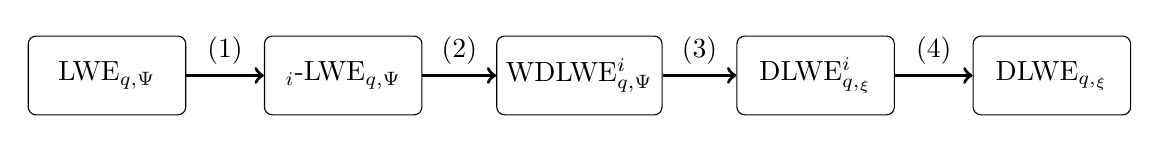
\begin{tikzpicture}
% Define the first acronym
	\node[draw, rounded corners=1mm, minimum width=2cm, minimum height=1cm] (A) at (0,0) {LWE$_{q, \Psi}$};

% Define the second acronym
	\node[draw, rounded corners=1mm, minimum width=2cm, minimum height=1cm] (B) at (3,0) {$\q_i$-LWE$_{q, \Psi}$};

% Define the third acronym
	\node[draw, rounded corners=1mm, minimum width=2cm, minimum height=1cm] (C) at (6,0) {WDLWE$^i_{q, \Psi}$};

% Define the fourth acronym
	\node[draw, rounded corners=1mm, minimum width=2cm, minimum height=1cm] (D) at (9,0) {DLWE$^i_{q, \D_{\xi}}$};

% Define the fifth acronym
\node [draw, rounded corners=1mm, minimum width=2cm, minimum height=1cm] (E) at (12,0) {DLWE$_{q, \D_{\xi}}$};

% Draw the arrows between the acronyms
	\draw[->, very thick] (A.east) -- node [above] {(1)} (B.west);
	\draw[->, very thick] (B.east) -- node [above] {(2)} (C.west);
	\draw[->, very thick] (C.east) -- node [above] {(3)} (D.west);
	\draw[->, very thick] (D.east) -- node [above] {(4)} (E.west);
\end{tikzpicture}
\caption{Schematic of reductions from R-LWE to R-DLWE}
\label{fig:4reds}
\end{figure}

\paragraph{Search to Worst-Case Decision}
We begin with the reduction of the LWE to $\q_i$-LWE distribution relative to only one $\q_i$ arbitrary prime ideal.
\begin{definition}
	The $\q_i$-LWE$_{q,\Psi}$ problem is: given access to A$_{s,\Psi}$ for some arbitrary $s \in \Rd_q$ and $\psi \in \Psi$, find $s \mod \q_i R$.
\end{definition}
\begin{lemma}[LWE to $\q_i$-LWE, Lemma 5.5 \cite{ring-lwe}]
	Suppose that the family $\Psi$ is closed under all the automorphisms of $K$, i.e., $\psi \in \Psi \Rightarrow \tau_k(\psi) \in \Psi$ for every $k \in \Z^*_m$. Then for every $i \in \Z^*_m$, there is a deterministic polynomial-time reduction from LWE$_{q, \Psi}$ to $\q_i$-LWE$_{q, \Psi}$.
\end{lemma}

\begin{proof}
	By assumptions, we are given access to an $\q_i$-LWE oracle along with $n$ field automorphisms $\tau_k$ that ``act transitively'' on the prime ideals $\q_i$ thanks to the underlying field being a cyclotomic number field. The idea is to use the oracle to recover the value of $s$ relative to every $\q_j\Rd$ using the automorphisms. Once we have that, we can (efficiently) recover the $s$ using the Chinese Remainder Theorem. 

	The reduction to find $s \mod \q_j \Rd$ works as follows: transform each given sample $(a,b) \leftarrow \text{A}_{s, \psi}$ to $(\tau_k(a), \tau_k(b)) \in R_q \cross \T$ where $k = j/i \in \Z^*_m$ which gives $\tau_k(\q_j) = \q_i$. Give the transformed sample to the oracle which outputs some $t \in \Rd / \q_i \Rd$. Since $\tau_k$ is a bijection, we can compute $\tau^{-1}_k(t) \in \Rd / \q_j \Rd$.

	We now need to verify that this output is actually equal to $s \mod \q_j \Rd$. This is equivalent to asking if $(\tau_k(a), \tau_k(b))$ is distributed according to A$_{\tau_k(s), \psi '}$ for $\psi ' = \tau_k(\psi)$. First, note that the automorphisms fix the underlying structure. Namely, $\tau_k(\Rd) = \Rd$ and $\tau_k(\T) = \T = K_{\R}/\Rd$ and in particular, $\tau_k(q) = q$ for any $k \in \Z_m^*$. We therefore have
	\[ \tau_k(b) = \tau_k(as)/q + \tau_k(e) \mod \Rd.\]
	If $a$ was uniformly distributed, $\tau_k(a)$ will be as well. The pairs are therefore distributed according to A$_{\tau_k(s), \psi '}$ for $\psi ' = \tau_k(\psi) \in \Psi$. The $t$ returned by an oracle must therefore be $t = \tau_k(s) \mod \q_i \Rd$ and so $\tau_k^{-1}(t) = s \mod \tau_k^{-1}(\q_i \Rd) = s \mod \q_j \Rd$ as required. 

	All we need to show now is that the automorphisms preserve the distribution. The proof is short and omited from here but can be found as Lemma 5.6 in \cite{ring-lwe}. As an outline, recall that the automorphisms simply permute the coordinates of the canonical embedding. So for any $\D_{\bm{r}}$ with each $r_i \leq \alpha$, it is sent to $\D_{\bm{r'}}$ where $\bm{r'}$ is simply the permutation of coefficients of the vector $\bm{r}$ and so, each $r_i' \leq \alpha$. Thus $\tau_k(\D_{\bm{r}}) \in \Psi_{\leq \alpha}$ as required.
\end{proof}


Chinese remainder theorem for rings --> Thm II.4.12 in Top's lecture notes. \\
For instance, they have unique factorization of ideals, and their fractional ideals form a multiplicative group; in general, neither property holds in $\Z[x]/\langle f (x) \rangle$ for monic irreducible $f (x)$, as demonstrated by the ring $\Z[x]/\langle x^2+3 \rangle = \Z[\sqrt{-3}]$. (For example, in this ring $4 = 22 = (1+\sqrt{-3})(1 - \sqrt{-3})$, but 2, $1 + \sqrt{-3}$, and $1 - \sqrt{-3}$ are all irreducible.)
Toward basing fully homomorphic encryption on worst-case hardness \\
One of the applications is \cite{qTESLA} signature scheme.

\subsection{Fully Homomorphic Encryption Using Ideal Lattices}
three ``generations'' of fhe schemes, first original gentry, smart and
explain here how we can construct a really nice homomorphic encryption scheme using ideal lattices \cite{gentry}. present the 
\subsubsection*{On Ideal Lattices and Learning With Errors Over Rings}
this is somewhat too difficult for me i think so ill just present main findings without proofs and details \cite{regev}, \\
First explain what lattices are. \\
How do lattices relate to LWE? The secret key is associated with a random vector. \\
then show how ring-lwe satisfies both of our requirements \cite{ring-lwe}, namely, the believed hardness for quantum computers (SVP or approximate SVP) and FHE. Show also the problem with ring-LWE because the lattices that are used there are ideal lattices which obviously possess more structure than "normal" lattices.
